\documentclass[a4paper, 11pt, twocolumn]{article}
\usepackage[utf8]{inputenc}
\usepackage{graphicx}
\usepackage[unicode, colorlinks, hypertexnames=false, citecolor=red]{hyperref}
\usepackage{biblatex}
\addbibresource{ref.bib}

\begin{document}

\twocolumn[
		\begin{@twocolumnfalse}
			\begin{center}
				{\Large
					Vysoké učení technické v~Brně \\
					Fakulta informačních technologií \\
				}
				{
\includegraphics[width=0.6 \linewidth]{img/logo.png}} \\

				{\LARGE
					Microprocessors and Embedded Systems \\
					Project\,--\,Heart rate measurement \\(analog sensor) \\
				}
				\vspace{0.3cm}

				{\large
					Vladislav Sokolovskii (xsokol15) \\
					\texttt{xsokol15@stud.fit.vutbr.cz} \\
					\today
				}
			\end{center}
		\end{@twocolumnfalse}
	]

\section{Introduction}

Within this project you can get acquainted with I2C hardware protocol, how to read analog input and convert it to the digital form using embedded ADC component. This project was implemented in \texttt{Espressif IDF} framework using \texttt{VSCode} extension called \texttt{PlatformIO}. Presentation of project can be seen in \href{https://youtu.be/JHA2dlhXHdE}{this video}.

\vspace{-0.5cm}
\section{Hardware}

First of all, ground and power voltage were connected to the breadboard bus strips. Then hardware components were connected to the breadboard and tested with Arduino examples\cite{arduino_heart} \cite{arduino_oled}. The detailed explanation of the connection of single hardware components is demonstrated in the attached \href{https://youtu.be/JHA2dlhXHdE}{video}.
\begin{table}[ht]
		\begin{tabular}{p{2.5cm} p{2.3cm} p{1.9cm}}
			\hline
			Peripheral pin & ESP32 pin & Name in the code\\ \hline
			OLED~Vcc & 3V3 & -- \\
			OLED~GND   & GND & -- \\
			OLED~SCL   & IO22 & SCL\_PIN \\
			OLED~SDA   & IO21 & SDA\_PIN \\
			Sensor~Vcc   & 3V3 & -- \\
			Sensor~GND   & GND & -- \\
			Sensor~Signal   & IO36 & channel \\
		\end{tabular}

		\caption{Hardware connection}
		\label{tab:hardware_connection}
	\end{table}
	\\
\subsection{OLED dsiplay SSD1306}

From the table you can tell that the display is connected to the MCU via \texttt{SCL} and \texttt{SDA} pins, hence, I2C Physical Protocol is used for the communication. Initial I2C setup is described in \texttt{i2c\_master\_init()} function.

In order not to program the display by pixel from scratch an open source sample code was used. This repository\footnote{\url{https://github.com/yanbe/ssd1306-esp-idf-i2c}} provides the display initialization function \texttt{ssd1306\_init()} and by-pixel definition of all \texttt{ASCII} symbols \texttt{font8x8\_basic.h}. Using this library writing something to the display is as easy as providing a string to the \texttt{task\_ssd1306\_display\_text()} function.

\subsection{Pulse sensor}

The working principle of pulse sensor is very simple. When you put a finger on the sensor it emits green light,
when the heart is pumping there is a flow of blood in veins. The light sensor will receive more light when the blood flow is sensed, this small change is enough to see the periodicity of incoming signal and count beats per minute.\par
The signal coming from sensor has very high frequency and noise so multisampling is used to make it more appropriate for the heart beat measurement. Current voltage on the sensor is calculated as average value over 200 measurements \texttt{read\_sensor\_voltage()}. The built-in Analog to Digital Converter is used \texttt{esp\_adc\_cal\_raw\_to\_voltage()} to convert raw signal to voltage.


\section {Implementation}
Project was partially implemented according to the examples provided by Espressif Systems Github page\footnote{\url{https://github.com/espressif/esp-idf/tree/master/examples}}. Official Espressif documentation was a good source of relevant informarion as well\cite{esp-doc}.

\subsection{Beats Per Minute}
The BPM is calculated over the last \texttt{samples\_number}, the number of samples is a pseudo randomly generated number from \newline[55; 65] interval. Randomness is used to avoid the case when the periodical signal is always cut at the same place of its period. Peak detection algorithm\footnote{\url{https://www.baeldung.com/cs/signal-peak-detection}} is used to count the number of heart beats over the given signal \texttt{get\_bpm()}. For verifying the signal, auxiliary python script for plotting the signal was implemented. In the graph (Fig. 1) you can see pronounced periodicity of heart beats.
\begin{figure}[]
    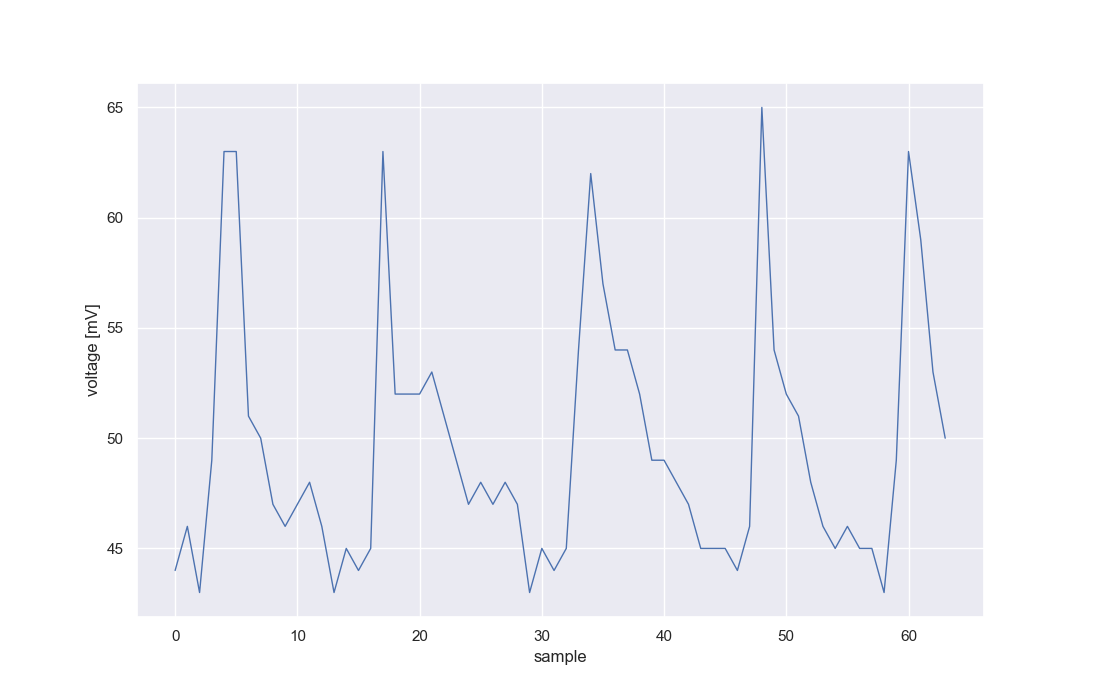
\includegraphics[scale=0.3]{img/heart_beats.png}
    \caption{Voltage from sensor (finger is on)}
    \label{graph}
\end{figure}
Number of peaks is converted to BPM using the following formula:
\[ BPM = round(\frac{60}{t\_period\_in\_sec} * peaks) \]
\par
Current BPM is stored to \texttt{bpm\_window[]} circular buffer of \texttt{BPM\_WINDOW\_SIZE} integers.
After getting the first valid BPM value the result is written to the display. The resulting BPM is calculated as an average value over the legit measurements stored in the buffer. The longer finger is placed on the sensor the more accurate the result becomes. When the current BPM becomes lower than \texttt{MINIMUM\_HEART\_RATE} it means that finger was removed from the sensor (or finger was not still), the buffer is cleared and \texttt{"Put your finger on sensor"} message is displayed. In order to get the accurate result you should not move your finger or press on sensor during the measurement.

Since sensor is calculating the reflection of green light, you can just wave in front of the sensor and it will detect some periodic signal and display the "waves per minute". Also, it was noticed that during the night time when there is no any ambient light the sensor produces pretty noisy signal, there should be a physical explanation to this phenomena.

\subsection{Display}

The messages are transported to the display via I2C protocol. Before starting the communication the command link has to be created \texttt{i2c\_cmd\_link\_create()}, then according to the protocol master has to transmit START signal to the given commands link \texttt{i2c\_master\_start()} to initiate the communication. After initializing the command link the communication can start \texttt{i2c\_master\_write()}, when all data is transmitted the link has to be terminated with the STOP signal \texttt{i2c\_master\_stop()}.
\par
As mentioned above it was decided to use open source by-pixel declaration of every \texttt{ASCII} symbol. However, an attempt was made to display non \texttt{ASCII} heart symbol, which you can see in the \href{https://youtu.be/JHA2dlhXHdE}{video}. Every symbol is coded in 8 hexadecimal numbers where each bit represents one pixel on the screen. For instance, "H" is coded as \newline \texttt{[ 0x7F, 0x7F, 0x08, 0x08, 0x7F, 0x7F, 0x00, 0x00 ]} and if you covert it to binary you will see rotated "H" letter:\\
0\textbf{1111111}\\
0\textbf{1111111}\\
0000\textbf{1}000\\
0\textbf{1111111}\\
0\textbf{1111111}\\

According to this pattern heart symbol was divided to 4 sections each represents quarter of the heart, these 4 \texttt{ASCII} symbols \texttt{@=?>} were redefined in \texttt{font8x8\_basic.h}.
\begin{figure}[h]
    
\includegraphics[scale=0.4]{img/heart.jpg}
    \caption{By pixel heart symbol}
    \label{graph}
\end{figure}


After connecting MCU to the power supply \texttt{"Put your finger on sensor"} message is displayed
on the display. This message will change to the number of heart beats per minute only after reasonable BPM is detected on sensor.

\section{Conclusion}
\subsection{Summary}
The chosen method of calculating the heart beats is not ideal but sufficient enough. The application results were compared with \texttt{"HeartRate"} application for `iOS` and difference of measurements was in the interval [-2;+4]. In the attached \href{https://youtu.be/JHA2dlhXHdE}{video} you can see sensor detecting heart rate growth after the exercise and code go-through. In the description there are some time codes for your convenience.\\

\url{https://youtu.be/JHA2dlhXHdE}

\onecolumn
\subsection{Self-evaluation}
\begin{itemize}
  \item \textbf{F} - functionality, result is satisfying, slight deviation is present \textbf{5}
  \item \textbf{Q} - quality, source code is commented, problem was divided to sub-problems \textbf{3}
  \item \textbf{P} - presentation, \href{https://youtu.be/JHA2dlhXHdE}{video} is good and clear \textbf{3}
  \item \textbf{D} - documentation, is detailed and clear \textbf{3}
  \item \textbf{E} - approach \textbf{1}
\end{itemize}
Expected: 13.5 - 14 points

 % -------------------------------------------------------------------
    % Bibliography/References  -  Harvard Style was used in this report
    % -------------------------------------------------------------------
    
    \printbibliography[heading=bibintoc]
\end{document}
